\documentclass[a4paper, 12pt]{article}%тип документа

%отступы
\usepackage{multirow}
\usepackage[left=2cm,right=2cm,top=2cm,bottom=3cm,bindingoffset=0cm]{geometry}

%Русский язык
\usepackage[T2A]{fontenc} %кодировка
\usepackage[utf8]{inputenc} %кодировка исходного кода
\usepackage[english,russian]{babel} %локализация и переносы

%Вставка картинок
\usepackage{graphicx}
\graphicspath{{pictures/}}
\DeclareGraphicsExtensions{.pdf,.png,.jpg}

%Графики
\usepackage{pgfplots}
\pgfplotsset{compat=1.9}

%Математика
\usepackage{amsmath, amsfonts, amssymb, amsthm, mathtools}

%Заголовок
\author{Валеев Рауф Раушанович \\
группа 825}
\title{\textbf{Работа 2.5.1\\
Измерение поверхностного натяжения жикости}}

\begin{document}
\maketitle
\newpage
\section*{Цель работы}

	1) измерение температурной зависимости  коэффициента поверхностного натяжения дистиллированной воды с использованием известного коэффициента поверхностного натяжения спирта; 2) определение полной поверхностной энергии  и теплоты, необходимой для изотермического образования единицы  поверхности жидкости  при различной температуре. 
\section*{Краткая теоретическая справка}

	Наличие поверхностного слоя приводит к различию давлений по разные стороны от искривленной границы раздела двух сред.  Для сферического пузырька с воздухом  внутри жидкости избыточное давление даётся формулой Лапласа:
\[\Delta P = P_{in} - P_{out} = \dfrac{2 \sigma}{r} \]
где $\sigma$ - коэффициент поверхностного натяжения, $P_{in}$ и $P_{out}$ - давление внутри пузырька и снаружи, $r$ - радиус кривизны поверхности раздела двух фаз. Эта формула лежит в основе предлагаемого метода определения коэффициента поверхностного натяжения жидкости. Измеряется давление $\Delta P$, необходимое для выталкивания в жидкость пузырька воздуха.
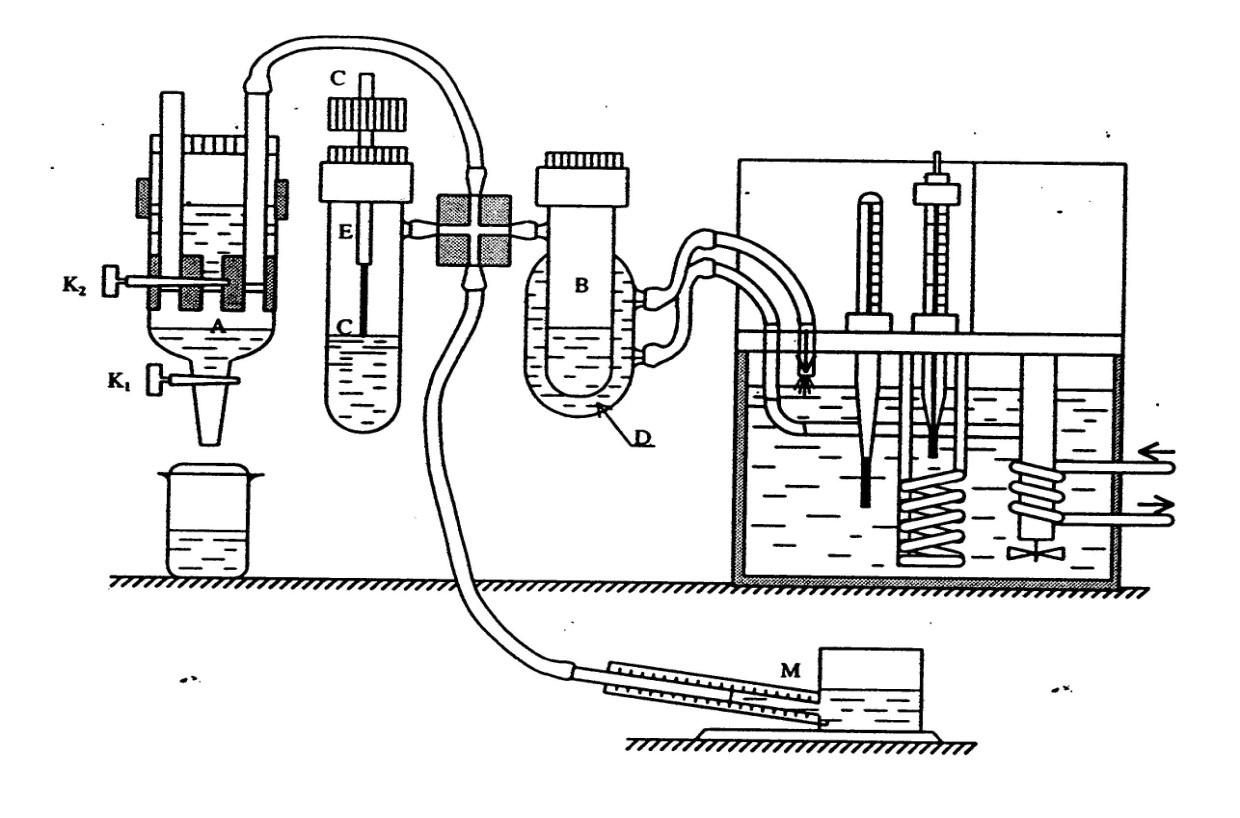
\includegraphics[width = 0.9\textwidth]{251_1.jpg}
\section*{Ход работы}

Измеряем максимальное давление $\Delta P_{alcohol}$  при  пробулькивании пузырьков воздуха через спирт. Записываем все в таблицу. Измеряем диаметр иглы по микроскопу, так же записываем в таблицу. Измеряем диаметр, полученный при измерении разности давлений спирта по формуле $d = \dfrac{4 \sigma}{\Delta P}$

\begin{tabular}{|c|c|c|c|}
\hline
$\Delta P$, Па              & $\sigma_{\Delta P}$, Па              & $d$, мм              & $\sigma_{d}$, мм              \\ \hline
82,4                        & 2                                    & 1,10                 & 0,03                          \\ \hline
80,1                        & 2                                    & 1,13                 & 0,03                          \\ \hline
84,7                        & 2                                    & 1,07                 & 0,03                          \\ \hline
82,4                        & 2                                    & 1,10                 & 0,03                          \\ \hline
\multicolumn{4}{|c|}{ $\overline{d_{alcohol}} = (1,1 \pm 0,3)$ мм, $d_{microscope} = (1,1 \pm 0,05)$ мм} \\ \hline
\end{tabular}

Измеряем при комнатной температуре $h_1$ и $h_2$ относительно какой-нибудь неподвижной детали, и измеряем $P_{1max}$ и $P_{2max}$ по $\Delta P$ найдем $\Delta h$ и сравним с $h_1 - h_2$. Учитываем, что при подсчете мы измеряем с помощью монометра $P = \Delta P + \rho g \Delta h$. Записываем результаты в таблицу.
\begin{center}
\begin{tabular}{|c|c|c|c|}
\hline
$P_1$, Па             & $h_1$, см            & $P_2$, Па            & $h_2$, см            \\ \hline
274                   & 1,8                  & 363                  & 0,8                  \\ \hline
274,7                 & 1,8                  & 360                  & 0,8                  \\ \hline
273,3                 & 1,8                  & 365                  & 0,8                  \\ \hline
265                   & 1,8                  & 363                  & 0,8                  \\ \hline \hline
271,75                & 1,8                  & 362,75               & 0,8                  \\ \hline
\multicolumn{4}{|c|}{$h_1 - h_2 = 1$ см, $\dfrac{P_2 - P_1}{\rho g} = (0,93 \pm 0,2)$ см} \\ \hline
\multicolumn{4}{|c|}{$\rho g \Delta h = (91 \pm 2,5)$ Па}                                  \\ \hline
\end{tabular} \\
\begin{tabular}{|c|c|c|c|c|c|}
\hline
$T$, K & $P$, Па & $\sigma_P$, Па & $\Delta P$, Па & $\sigma_{water} \cdot 10^{-3}$, Н/м & $\sigma_{\sigma_{water}} \cdot 10^{-3}$, Н/м \\ \hline
25,00  & 364,00  & 2,00           & 273,00    & 75,08                               & 0,5                                        \\ \hline
30,00  & 362,00  & 2,00           & 271,00    & 74,53                               & 0,5                                        \\ \hline
35,00  & 359,00  & 2,00           & 268,00    & 73,70                               & 0,5                                        \\ \hline
40,00  & 357,00  & 2,00           & 266,00    & 73,15                               & 0,5                                        \\ \hline
45,00  & 353,00  & 2,00           & 262,00    & 72,05                               & 0,5                                        \\ \hline
50,00  & 350,00  & 2,00           & 259,00    & 71,23                               & 0,5                                        \\ \hline
55,00  & 347,00  & 2,00           & 256,00    & 70,40                               & 0,5                                        \\ \hline
60,00  & 343,00  & 2,00           & 252,00    & 69,30                               & 0,5                                        \\ \hline
50,00  & 345,00  & 2,00           & 254,00    & 69,85                               & 0,5                                        \\ \hline
45,00  & 347,00  & 2,00           & 256,00    & 70,40                               & 0,5                                        \\ \hline
30,00  & 350,00  & 2,00           & 259,00    & 71,23                               & 0,5                                        \\ \hline
\end{tabular}
\end{center}
\newpage
Представляем данные в виде графика и находим $\dfrac{d \sigma}{dT}$\\
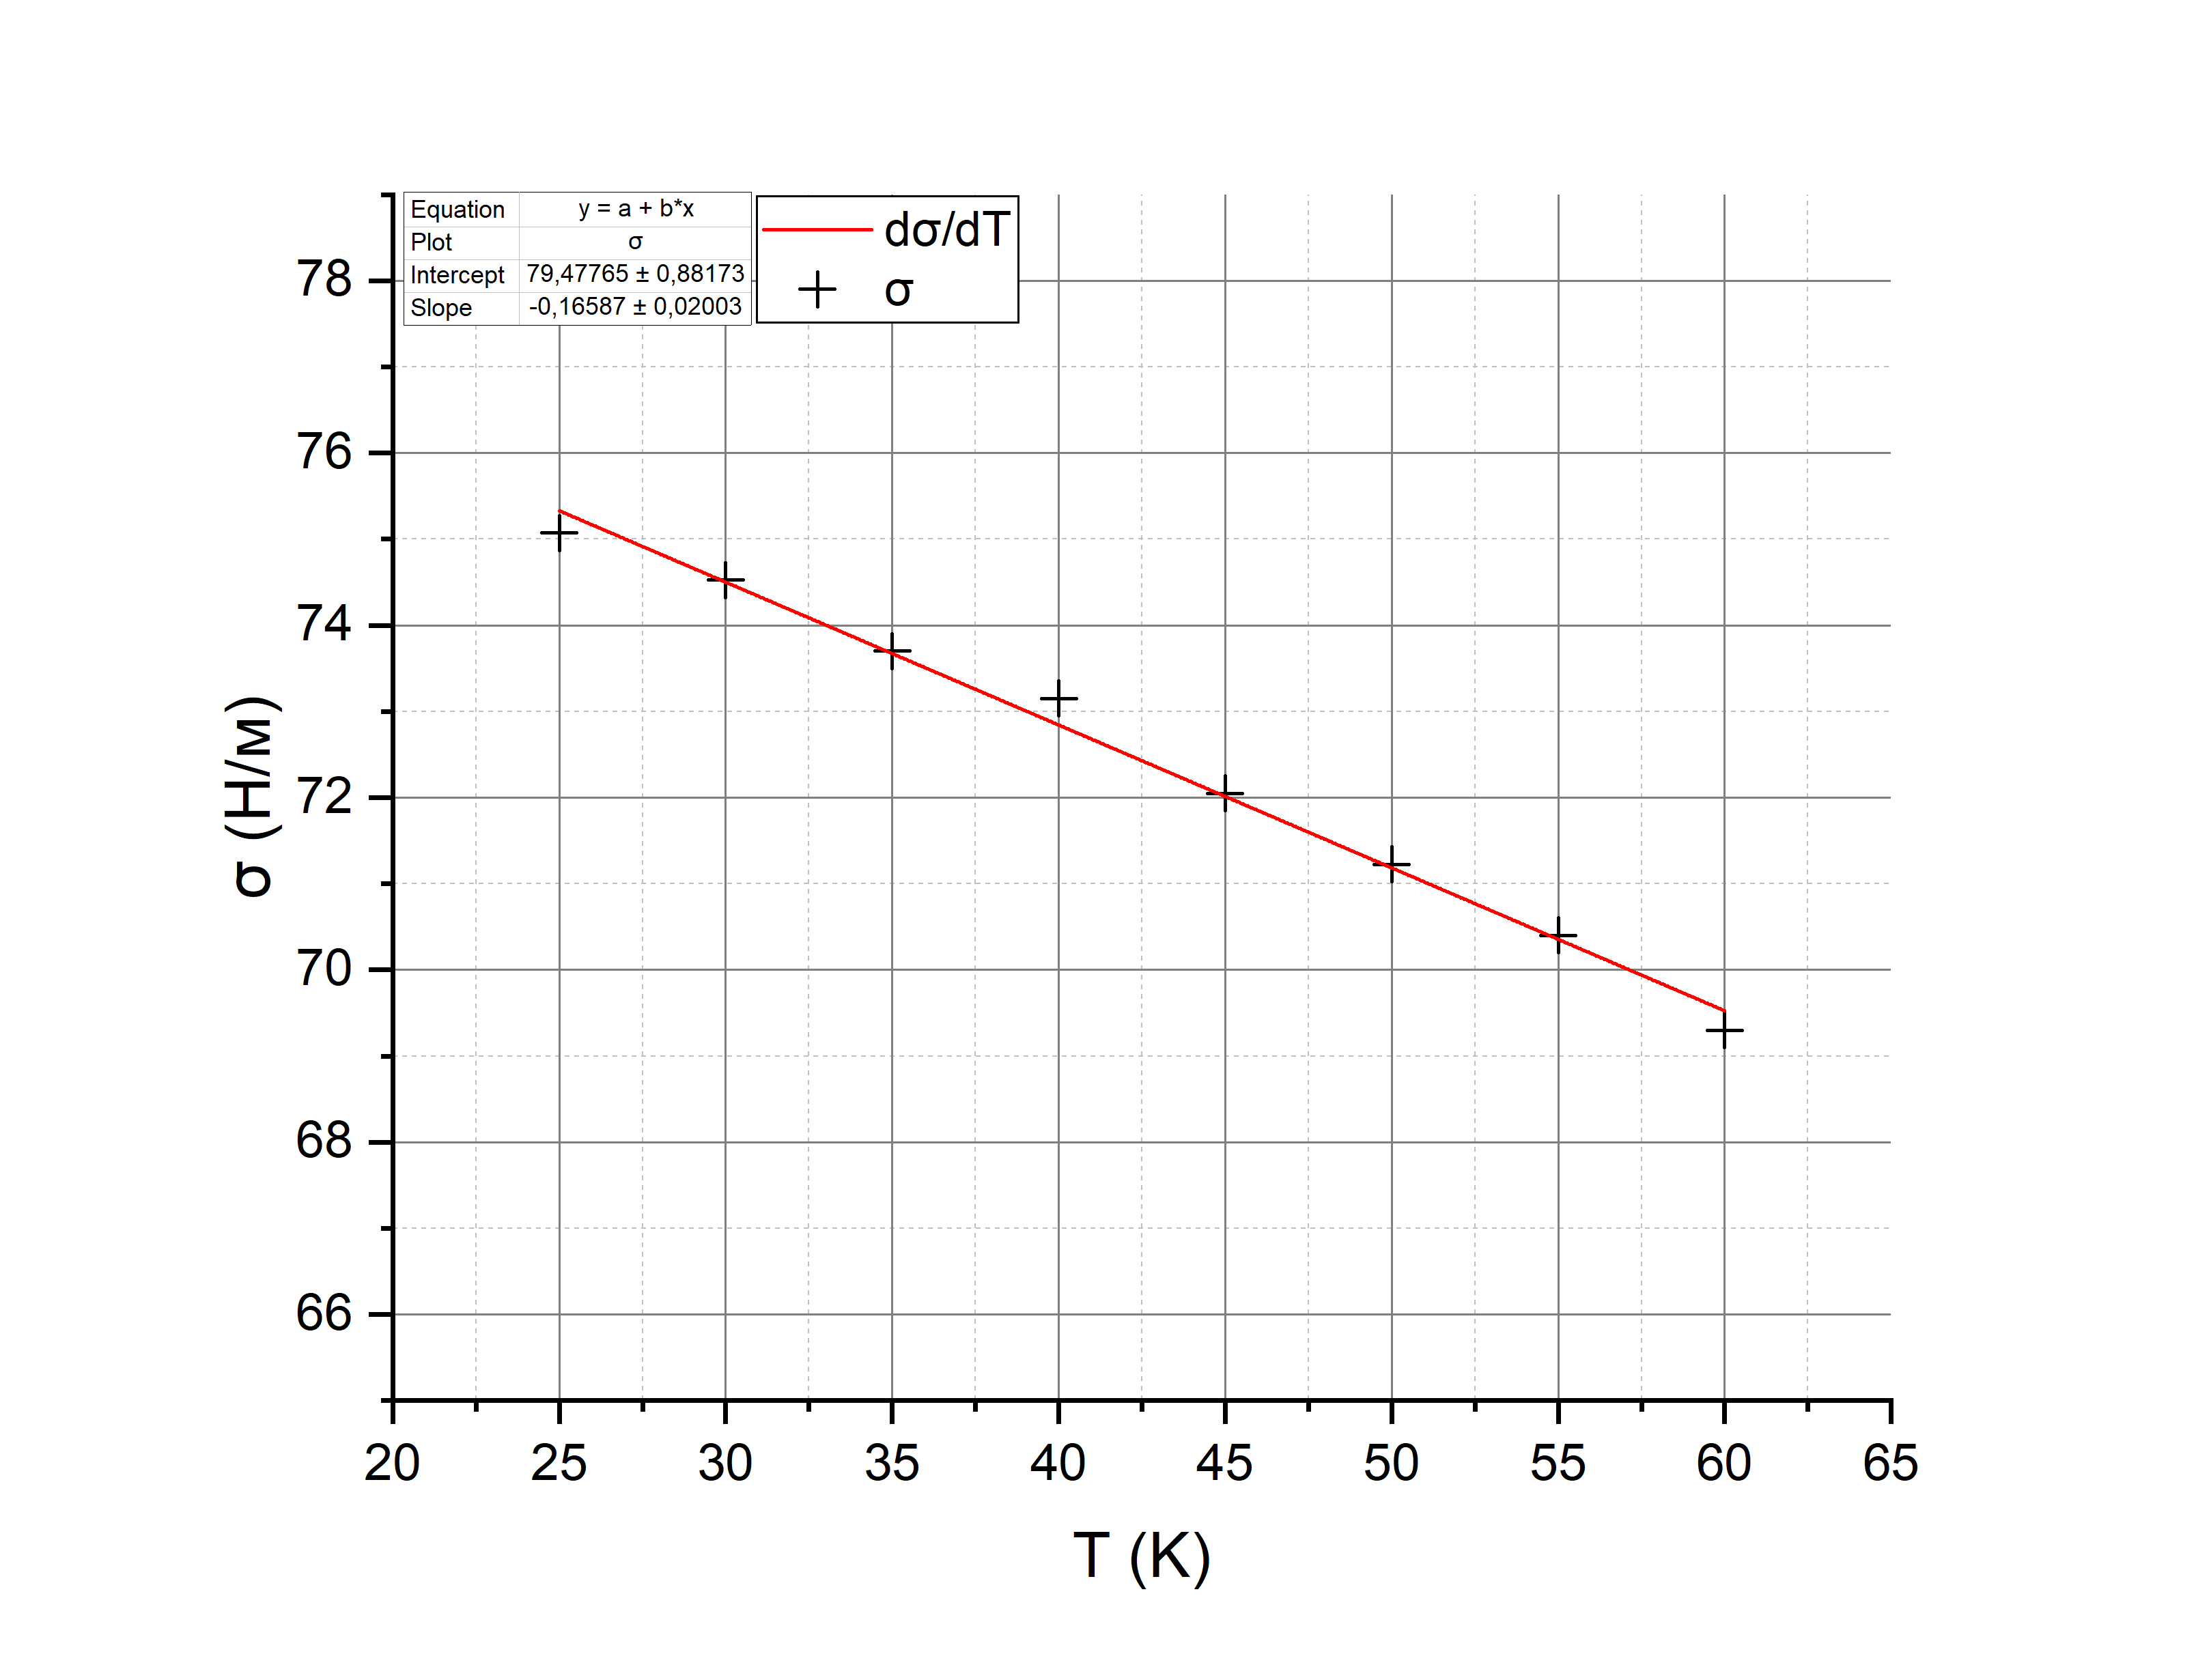
\includegraphics[width = 0.9\textwidth]{251_2.jpg}\\
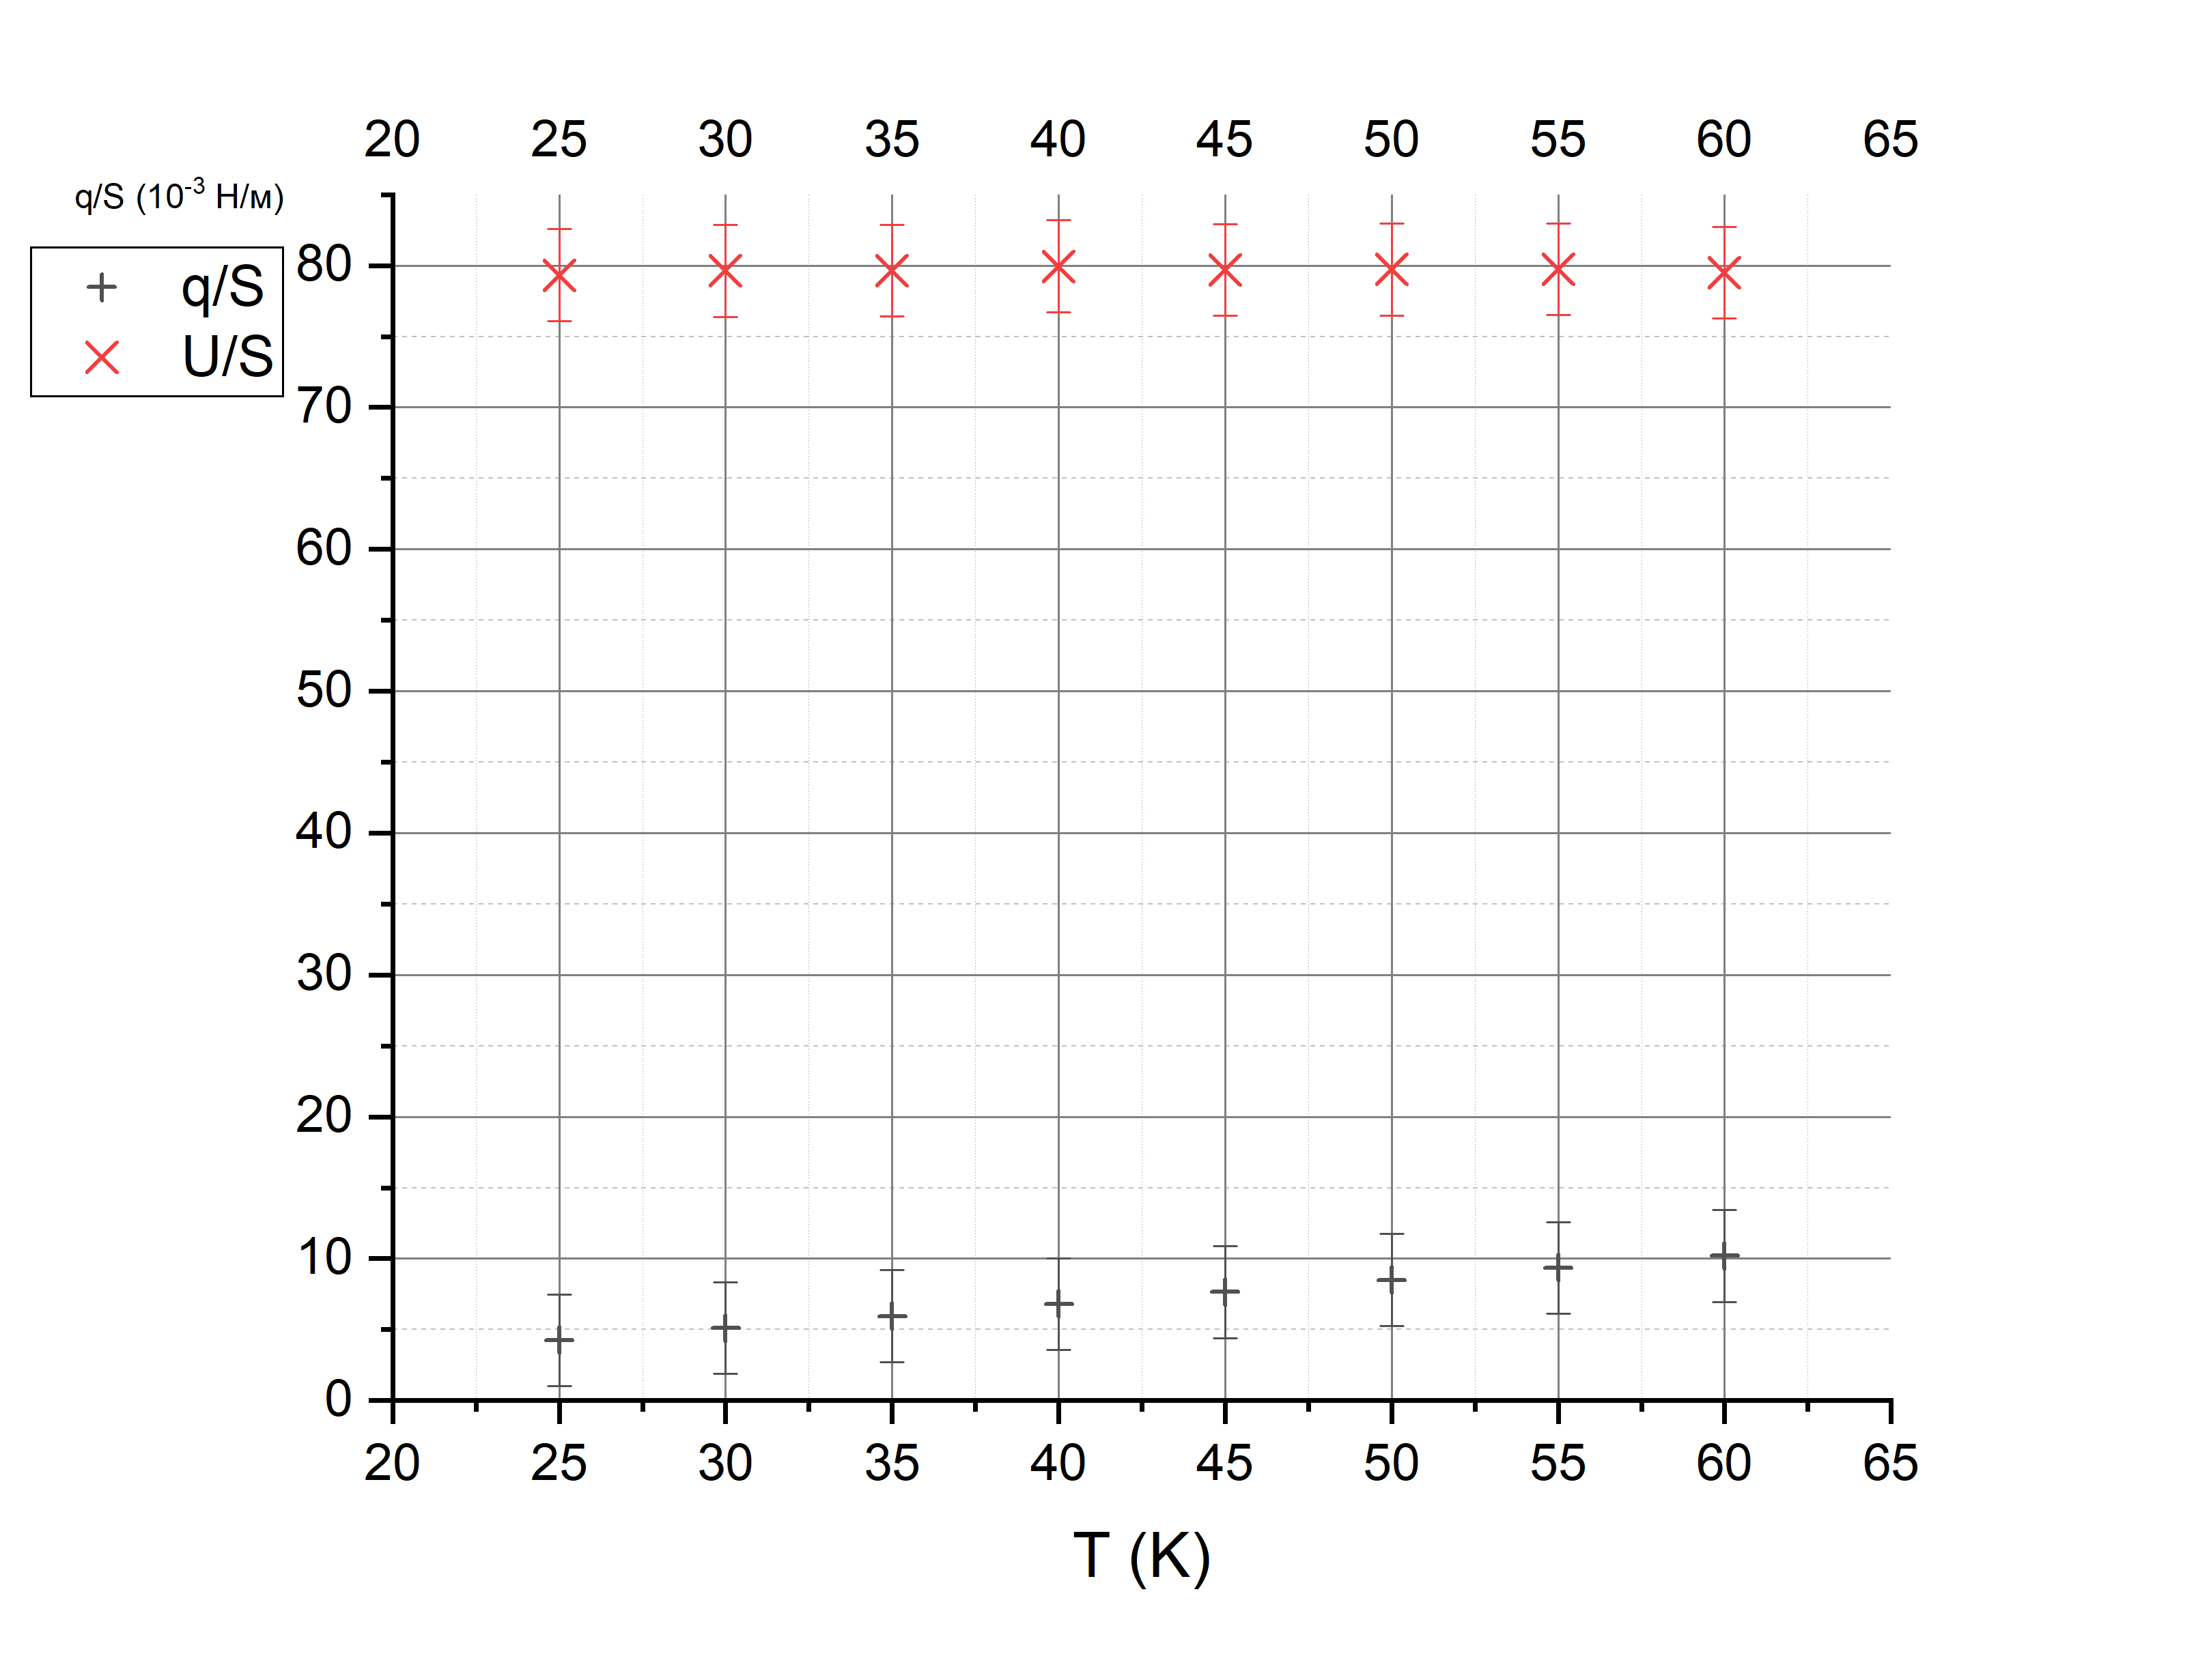
\includegraphics[width = 0.9\textwidth]{251_3.jpg}
\end{document}